\chapter{Results}
\label{sec:experiments}
%\begin{itemize}
%    \item In order to show correctness of implementation will solve a problem with two different RHS.
%    \item Explain the entire problem setup.
%    \item Create plot showcasing the convergence.
%    \item Show 2d plot of the solution.
%    \item Create some scaling study with strong and weak scaling for different problem sizes in both 2d and 3d.
%\end{itemize}

\section{Setup}
In this section we will test our implementation on one type of PDE, which is given by:
\begin{align}
    &\nabla \times \nabla \times \vec{u}(\vec{x}) + \vec{u}(\vec{x}) = \vec{g}(\vec{x}) \text{ in } \Omega \label{eq:strong}\\
    &\vec{u}(\vec{x}) \times \vec n =  \text{ on } \partial \Omega\text{,} \label{eq:boundary}
\end{align}
where \(\vec g (\vec x)\) is the source function, \(\vec u (\vec x)\) the solution, \(\vec n\) the domain normal (pointing outwards), and \(\Omega\) the domain with \(\partial \Omega\) being the boundary. For this PDE we define two different source functions \(\vec g(\vec x)\) and two different domains \(\Omega\). The first case, which we call ``Trigonometric'' has the following \(\vec g(\vec x)\) and \(\Omega\):
\begin{align}
    \vec{g}(\vec x) = 
    \begin{cases}
        \begin{bmatrix}
            (1+k^2)\sin(k y)\\ (1+k^2)\sin(k x)
        \end{bmatrix} & \text{ for 2D, with }\Omega=[1,3]^2\\
        \noalign{\vskip9pt}
        \begin{bmatrix}
            (1 + k^2)\sin(k y)\sin(k z) \\
            (1 + k^2)\sin(k x)\sin(k z) \\
            (1 + k^2)\sin(k x)\sin(k y)
        \end{bmatrix} & \text{ for 3D, with }\Omega=[1,3]^3\\
    \end{cases}\text{.}
\end{align}
The second case, which we call ``Polynomial'', has the following \(\vec g(\vec x)\) and \(\Omega\):
\begin{align}
    \vec{g}(\vec x) = 
    \begin{cases}
        \begin{bmatrix}
            2 - (y^2 - 1)\\ 2 - (x^2 - 1)
        \end{bmatrix}& \text{ for 2D, with }\Omega=[-1,1]^2\\
        \noalign{\vskip9pt}
        \begin{bmatrix}
            -2 (z^2 - 1) - 2 (y^2 - 1) + (y^2 - 1) (z^2 - 1) \\
            -2 (x^2 - 1) - 2 (z^2 - 1) + (x^2 - 1) (z^2 - 1) \\
            -2 (y^2 - 1) - 2 (x^2 - 1) + (x^2 - 1) (y^2 - 1)
        \end{bmatrix}& \text{ for 3D, with }\Omega=[-1,1]^3
    \end{cases}\text{.}
\end{align}
We then have that the exact solution \(\vec u (\vec x )\) for the Trigonometric problem is:
\begin{align}
    \vec{u}(\vec x) = 
    \begin{cases}
        \begin{bmatrix}
            \sin(k y)\\ \sin(k x)
        \end{bmatrix} & \text{ for 2D}\\
        \noalign{\vskip9pt}
        \begin{bmatrix}
            \sin(k y)\sin(k z) \\
            \sin(k x)\sin(k z) \\
            \sin(k x)\sin(k y)
        \end{bmatrix} & \text{ for 3D}\\
    \end{cases}\text{,}
\end{align}
and for the Polynomial one it is:
\begin{align}
    \vec{u}(\vec x) = 
    \begin{cases}
        \begin{bmatrix}
            - (y^2 - 1)\\ - (x^2 - 1)
        \end{bmatrix}& \text{ for 2D}\\
        \noalign{\vskip9pt}
        \begin{bmatrix}
            (y^2 - 1) (z^2 - 1) \\
            (x^2 - 1) (z^2 - 1) \\
            (x^2 - 1) (y^2 - 1)
        \end{bmatrix}& \text{ for 3D}
    \end{cases}\text{.}
\end{align}
\medskip

In order to solve the problem described by Equations (\ref{eq:strong}) and (\ref{eq:boundary}) using FEM we need to find its variational formulation. Luckily this is a very common type of problem and therefore this has already be done for us in \cite{maxwellBook}. The variational formulation is given by:
\begin{align}
    \int_{\Omega} \nabla \times \vec u(\vec x) \cdot \nabla \times \vec v(\vec x) d\vec x + \int_{\Omega} \vec u(\vec x) \cdot \vec v(\vec x) d\vec x = \int_{\Omega} \vec u(\vec x) \cdot \vec g(\vec x) d\vec x \text{, }\label{eq:varita}
\end{align}
where we enforce the zero dirichlet boundary by skipping DOFs located on the boundary. From this we now also can quite easily extract the \(\mathcal F (\cdot, \cdot)\) of Equation (\ref{eq:varlhs}):
\begin{align}
    \mathcal{F}\left(\vec u (\vec x), \vec v (\vec x)\right) = \nabla \times \vec u(\vec x) \cdot \nabla \times \vec v(\vec x) + \vec u(\vec x) \cdot \vec v(\vec x) \text{.}
\end{align}\medskip

During the element-based assembling scheme we are going to assemble the local matrices for the LHS and local parts of the vector for the RHS for every element in the mesh. In order to simplify calculations we are not going to work on the actual elements of the mesh, but rather on the reference element. In Section \ref{subsec:theory} we already introduced the transformations required, our problem transforms into:
\begin{align}
    & A_{i,j} = \int_{K} \nabla \times \vec \beta_i \cdot \nabla \times \beta_j d\vec x  + \int_{K} \vec \beta_i \cdot \vec \beta_j d\vec x = \int_{\hat K} J^{-T}(\nabla \times \hat{\vec\beta}_i) \cdot J^{-T} (\nabla \times \hat{\vec\beta}_j) d\vec x + \int_{\hat K} \hat{\vec\beta}_i \cdot \hat{\vec\beta}_j d\vec x \text{,}\\
    & s_{i} = \int_{K} \vec \beta_i \cdot \vec g(\vec x) d\vec x = \int_{\hat K} \hat{\vec\beta}_i \cdot \vec g(\vec x) d\vec x \text{,}
\end{align}
where $J^{-T}$ is the inverse transpose Jacobian of the affine transformation between the reference and the actual element.\medskip


\section{Correctness}
\begin{figure}
    \centering
    \begin{subfigure}{0.49\textwidth}
        \centering
        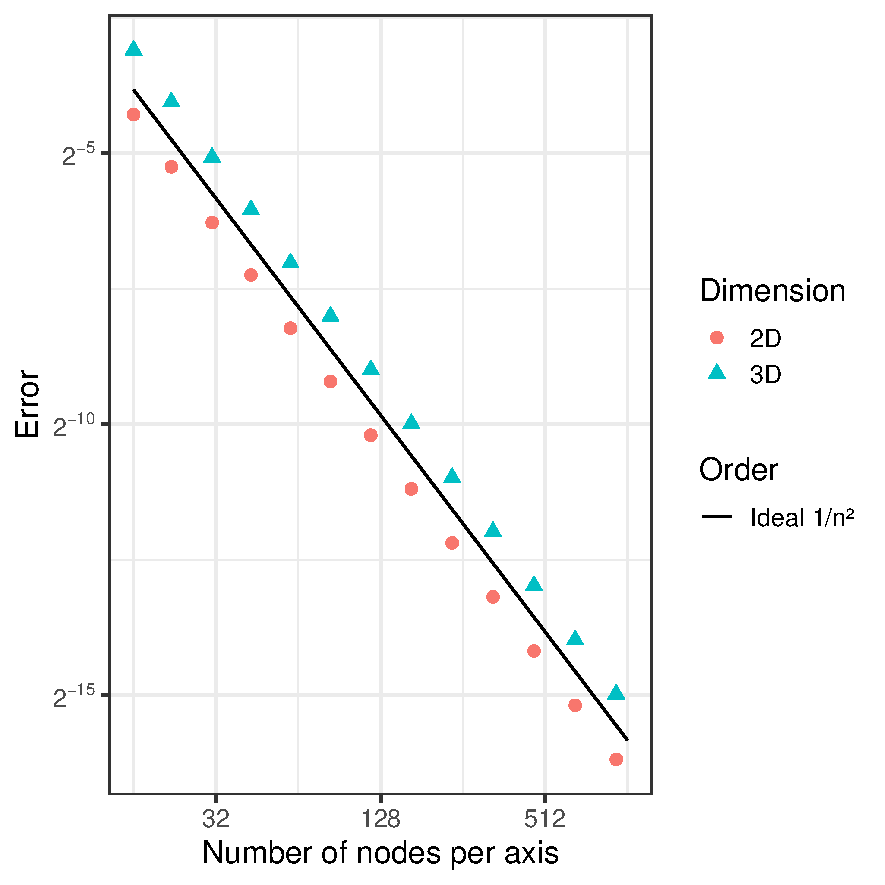
\includegraphics[width=\linewidth]{figures/experiments/convergence_trig.pdf}
        \caption{Trigonometric case.}
    \end{subfigure}
    \begin{subfigure}{0.49\textwidth}
        \centering
        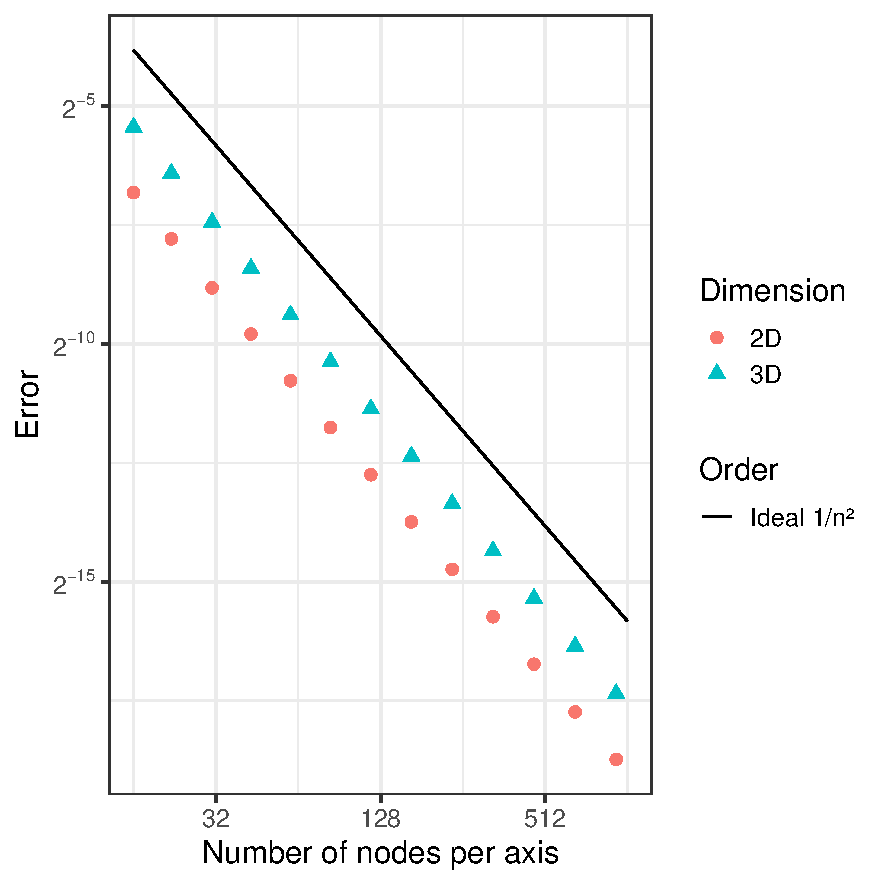
\includegraphics[width=\linewidth]{figures/experiments/convergence_poly.pdf}
        \caption{Polynomial case.}
    \end{subfigure}
    \caption{L2 error convergences for the different problems. As we can see, perfect order 2 convergence is achieved.}
    \label{fig:convergence}
\end{figure}
\begin{table}
    \centering
    \begin{subtable}{\textwidth}
        \centering
        \begin{Large}
            Trigonometric problem
        \end{Large}
        \begin{small}
            \begin{tabular}{ccc@{\hskip 1cm}cc}
                \toprule
                & \multicolumn{2}{c}{2D\hphantom{asdf}} & \multicolumn{2}{c}{3D} \\
                Num nodes & L2 Error & Iterations & L2 Error & Iterations \\
                \cmidrule(lr{1cm}){2-3}\cmidrule(r){4-5}
                \( 16\)   &  \(5.125\cdot 10^{-2}\)  & \(  13\)  &  \(1.168\cdot 10^{-1}\) & \(   5\) \\
                \( 22\)   &  \(2.626\cdot 10^{-2}\)  & \(  19\)  &  \(6.013\cdot 10^{-2}\) & \(   8\) \\
                \( 31\)   &  \(1.290\cdot 10^{-2}\)  & \(  29\)  &  \(2.961\cdot 10^{-2}\) & \(  15\) \\
                \( 43\)   &  \(6.586\cdot 10^{-3}\)  & \(  42\)  &  \(1.514\cdot 10^{-2}\) & \(  22\) \\
                \( 60\)   &  \(3.339\cdot 10^{-3}\)  & \(  61\)  &  \(7.682\cdot 10^{-3}\) & \(  35\) \\
                \( 84\)   &  \(1.688\cdot 10^{-3}\)  & \(  89\)  &  \(3.884\cdot 10^{-3}\) & \(  54\) \\
                \(118\)   &  \(8.495\cdot 10^{-4}\)  & \( 165\)  &  \(1.955\cdot 10^{-3}\) & \(  93\) \\
                \(166\)   &  \(4.272\cdot 10^{-4}\)  & \( 248\)  &  \(9.833\cdot 10^{-4}\) & \( 233\) \\
                \(234\)   &  \(2.142\cdot 10^{-4}\)  & \( 335\)  &  \(4.932\cdot 10^{-4}\) & \( 343\) \\
                \(330\)   &  \(1.074\cdot 10^{-4}\)  & \(1026\)  &  \(2.474\cdot 10^{-4}\) & \( 994\) \\
                \(466\)   &  \(5.379\cdot 10^{-5}\)  & \(1609\)  &  \(1.238\cdot 10^{-4}\) & \(2321\) \\
                \(659\)   &  \(2.686\cdot 10^{-5}\)  & \(2963\)  &  \(6.184\cdot 10^{-5}\) & \(3883\) \\
                \(931\)   &  \(1.345\cdot 10^{-5}\)  & \(4261\)  &  \(3.096\cdot 10^{-5}\) & \(6185\) \\
                \bottomrule
            \end{tabular}
        \end{small}
    \end{subtable}
    \vskip 1cm
    \begin{subtable}{\textwidth}
        \centering
        \begin{Large}
            Polynomial problem
        \end{Large}
        \begin{small}
            \begin{tabular}{ccc@{\hskip 1cm}cc}
                \toprule
                & \multicolumn{2}{c}{2D\hphantom{asdf}} & \multicolumn{2}{c}{3D} \\
                Num nodes & L2 Error & Iterations & L2 Error & Iterations \\
                \cmidrule(lr{1cm}){2-3}\cmidrule(r){4-5}
                \( 16\)   &  \(8.824\cdot 10^{-3}\)  & \(   7\)  &  \(2.293\cdot 10^{-2}\) & \(  23\) \\
                \( 22\)   &  \(4.502\cdot 10^{-3}\)  & \(  12\)  &  \(1.171\cdot 10^{-2}\) & \(  36\) \\
                \( 31\)   &  \(2.206\cdot 10^{-3}\)  & \(  19\)  &  \(5.741\cdot 10^{-3}\) & \(  56\) \\
                \( 43\)   &  \(1.125\cdot 10^{-3}\)  & \(  29\)  &  \(2.930\cdot 10^{-3}\) & \(  81\) \\
                \( 60\)   &  \(5.703\cdot 10^{-4}\)  & \(  43\)  &  \(1.485\cdot 10^{-3}\) & \( 119\) \\
                \( 84\)   &  \(2.882\cdot 10^{-4}\)  & \(  62\)  &  \(7.503\cdot 10^{-4}\) & \( 170\) \\
                \(118\)   &  \(1.450\cdot 10^{-4}\)  & \(  90\)  &  \(3.776\cdot 10^{-4}\) & \( 267\) \\
                \(166\)   &  \(7.291\cdot 10^{-5}\)  & \( 185\)  &  \(1.899\cdot 10^{-4}\) & \( 382\) \\
                \(234\)   &  \(3.657\cdot 10^{-5}\)  & \( 178\)  &  \(9.522\cdot 10^{-5}\) & \( 640\) \\
                \(330\)   &  \(1.834\cdot 10^{-5}\)  & \( 483\)  &  \(4.776\cdot 10^{-5}\) & \(1039\) \\
                \(466\)   &  \(9.181\cdot 10^{-6}\)  & \(1113\)  &  \(2.391\cdot 10^{-5}\) & \(2086\) \\
                \(659\)   &  \(4.585\cdot 10^{-6}\)  & \(2220\)  &  \(1.194\cdot 10^{-5}\) & \(3592\) \\
                \(931\)   &  \(2.295\cdot 10^{-6}\)  & \(3600\)  &  \(5.977\cdot 10^{-6}\) & \(5804\) \\
                \bottomrule
            \end{tabular}
        \end{small}
    \end{subtable}
    \caption{Tables with exact values of the convergence studies. Additionally the number of CG iterations is also given.}
    \label{tab:convergence}
\end{table}
In order to gauge the correctness of the implementation a convergence study is done. To this extend the problems are solved multiple times while increasing the mesh resolution, for each case the L2 error as described in Section \ref{subsubsec:error_metric} is calculated and the result is plotted. For these experiments we went with number of nodes per dimension in the range of \(16\) to \(931\), a Gauss Jacobi quadrature using 5 nodes per dimension for the numerical quadrature is used, and the linear system is solved using a non-preconditioned conjugate gradient algorithm with tolerance set to \(10^{-13}\) and maximum number of iterations set to \(10000\). The plots resulting from this can be seen in Figure \ref{fig:convergence} with exact values given in Table \ref{tab:convergence}. From theory we would expect the error to converge with a rate of $\Theta(n^{-2})$ where $n$ is the number of vertices per dimension. As we can see in the plots we have this convergence, as expected.\medskip


\section{Scaling Analysis}
\begin{figure}
    \centering
    \begin{subfigure}{0.49\textwidth}
        \centering
        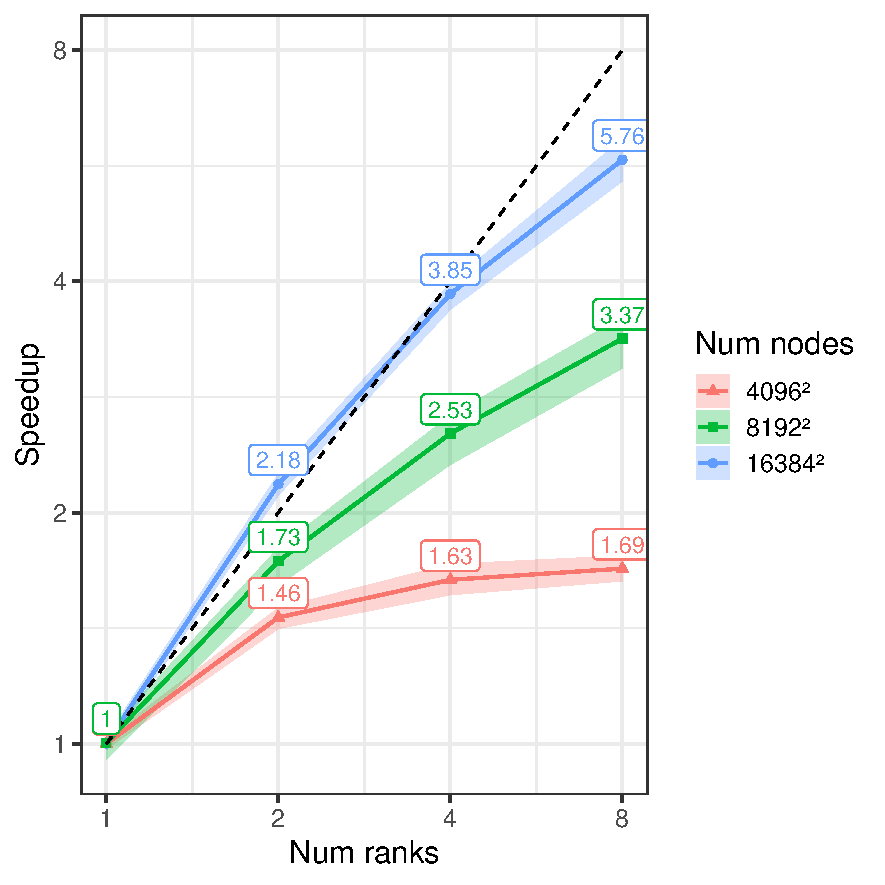
\includegraphics[width=\linewidth]{figures/experiments/scaling_strong_2d.pdf}
        \caption{2D case}
        \label{fig:scalingStrong2D}
    \end{subfigure}
    \begin{subfigure}{0.49\textwidth}
        \centering
        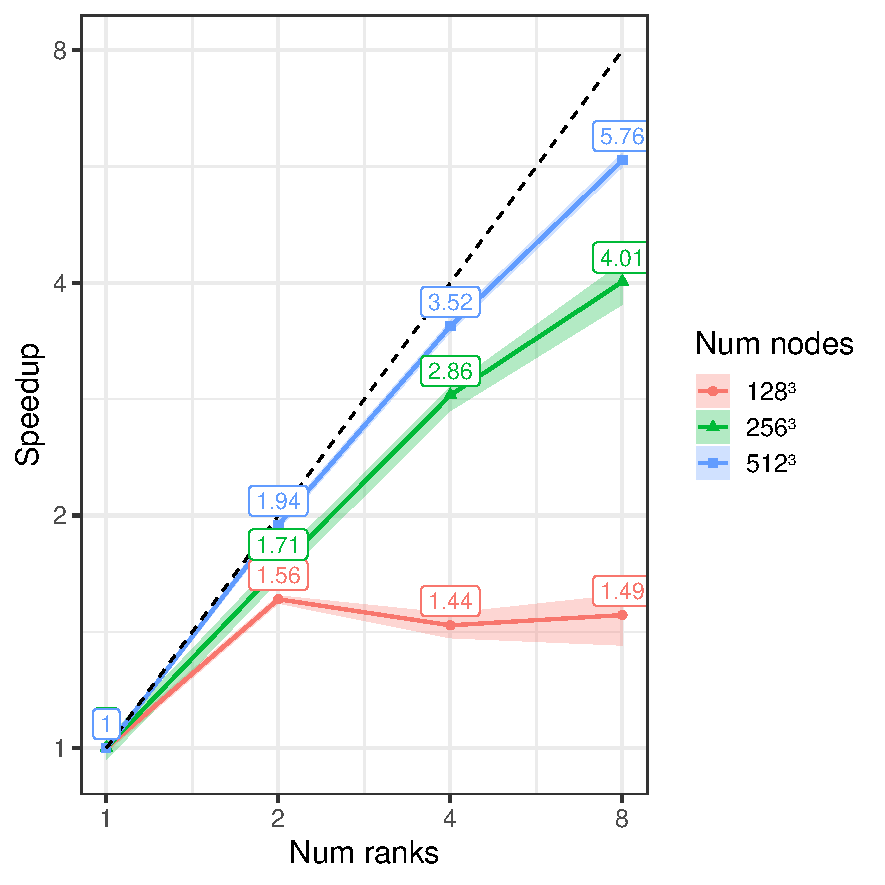
\includegraphics[width=\linewidth]{figures/experiments/scaling_strong_3d.pdf}
        \caption{3D case}
        \label{fig:scalingStrong3D}
    \end{subfigure}
    \caption{Strong scaling of the implementation. All runs where repeated 10 times with an additional warm-up run, mean and confidence intervals are plotted.}
    \label{fig:scalingStrong}
\end{figure}
\begin{figure}
    \centering
    \begin{subfigure}{0.49\textwidth}
        \centering
        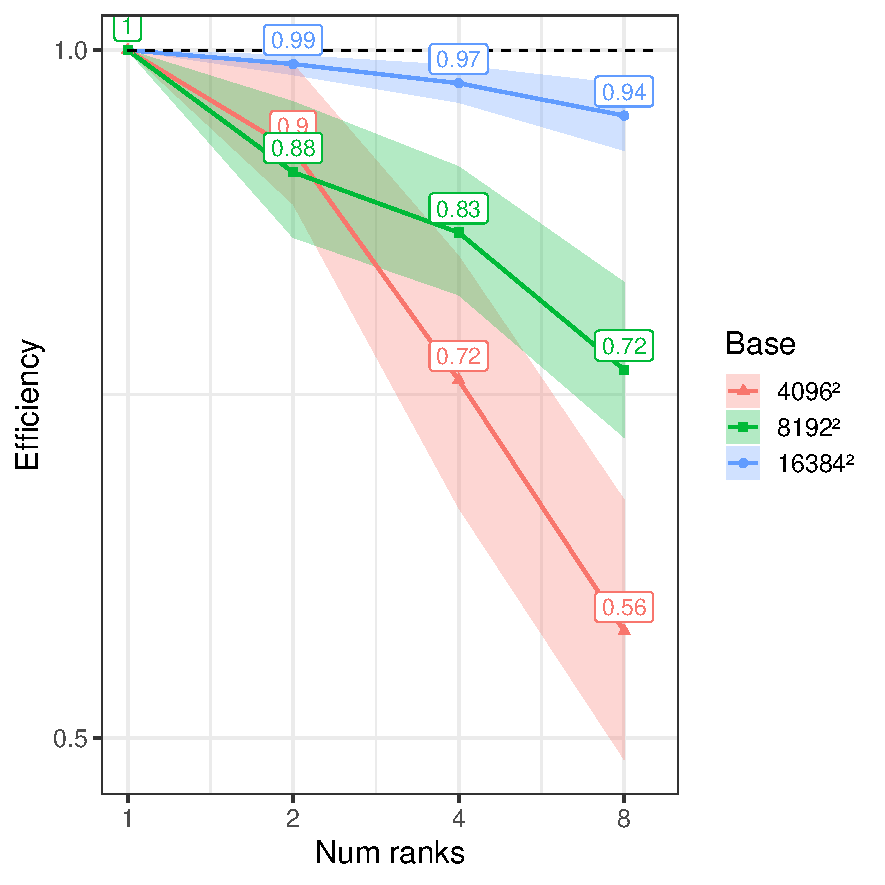
\includegraphics[width=\linewidth]{figures/experiments/scaling_weak_2d.pdf}
        \caption{2D case}
        \label{fig:scalingWeak2D}
    \end{subfigure}
    \begin{subfigure}{0.49\textwidth}
        \centering
        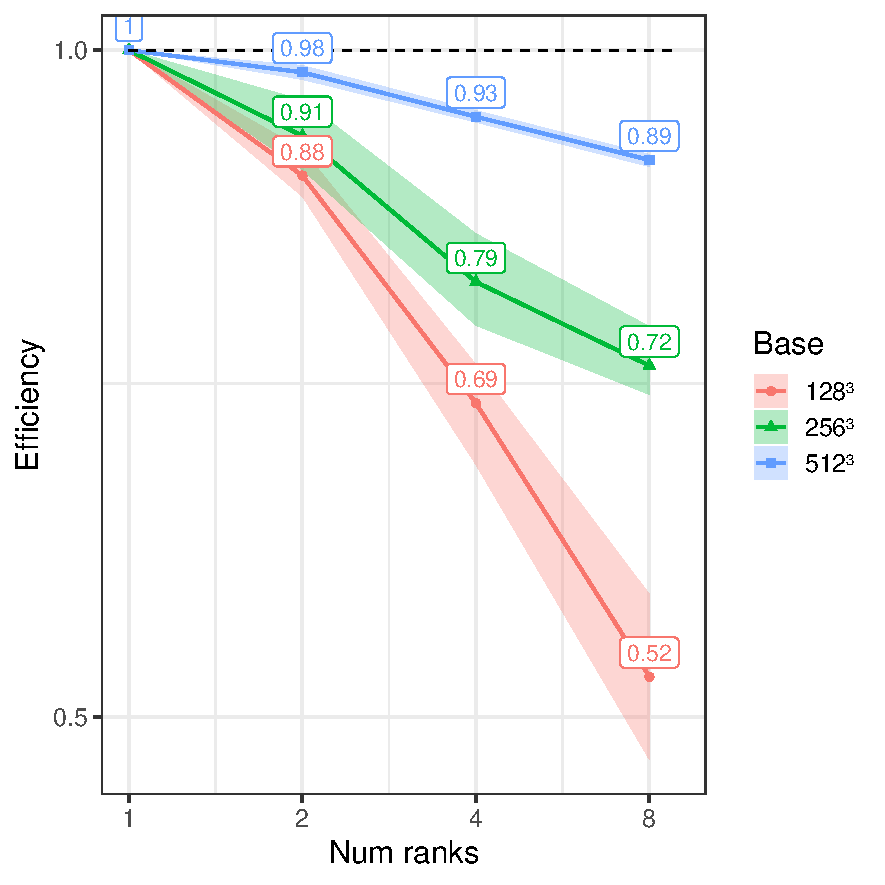
\includegraphics[width=\linewidth]{figures/experiments/scaling_weak_3d.pdf}
        \caption{3D case}
        \label{fig:scalingWeak3D}
    \end{subfigure}
    \caption{Weak scaling of the implementation. All runs where repeated 10 times with an additional warm-up run, mean and confidence intervals are plotted.}
    \label{fig:scalingWeak}
\end{figure}

\begin{table}
    \centering
    \begin{subtable}{0.49\textwidth}
        \begin{center}
\begin{tabular}{cc}
\toprule
\multicolumn{1}{c}{Num nodes}&\multicolumn{1}{c}{Time [s]}\tabularnewline
\midrule
$~4096$&$~0.6828832287$\tabularnewline
$~8192$&$~2.4991507782$\tabularnewline
$16384$&$11.3711869943$\tabularnewline
\bottomrule
\end{tabular}\end{center}

        \caption{2D case}
        \label{tab:time2d}
    \end{subtable}
    \begin{subtable}{0.49\textwidth}
        \begin{center}
\begin{tabular}{cc}
\toprule
\multicolumn{1}{c}{Num nodes}&\multicolumn{1}{c}{Time [s]}\tabularnewline
\midrule
$128$&$~0.7920425589$\tabularnewline
$256$&$~5.7699309643$\tabularnewline
$512$&$45.0464857090$\tabularnewline
\bottomrule
\end{tabular}\end{center}

        \caption{3D case}
        \label{tab:time3d}
    \end{subtable}
    \caption{Runtimes for for the scaling experiments in the case of a singular rank. The mean over the runs is calculated. Note that here in the case of a singular rank it does not matter if we consider the strong or the weak scaling case.}
\end{table}


We also perform a small scaling study of our implementation in the form of a strong and weak scaling analysis. The hardware setup we used for the runs consists of a two node setup, each equipped with a dual socket \(128\) core \texttt{AMD EPYC 7773X} and \(1\)TB of memory, and four \texttt{NVIDIA A100}s with \(80\)GB of memory each. For the network a \(200\)Gb/s Infiniband connection is used, and the MPI is a cuda aware \texttt{OpenMPI 5.0.3} instance, the operating system is \texttt{Rocky Linux 9.4}. For the runs we only consider the Polynomial case, as the performance between the two cases should be the same. It was configured identically to the previous section, with the exception that for both strong and weak scaling the maximum number of CG iterations are set to \(100\) and the tolerance is set to a negative value, like this we have that the number of CG iterations stays constant over the different domain sizes and therefore the work required is directly related to the domain size (which is critical for the weak scaling). All runs where repeated \(10\) times with an additional warm-up run for which then mean and confidence intervals are calculated. For strong scaling in 2D we went with problem sizes of \(4096^2\), \(8192^2\), and \(16384^2\) which where run with \(1\), \(2\), \(4\), and \(8\) ranks (where only for the case of \(8\) ranks we move to two nodes), this can be seen in Figure \ref{fig:scalingStrong2D}, with base runtimes in Table \ref{tab:time2d}. For the strong scaling in 3D we went with problem sizes of \(128^3\), \(256^3\), and \(512^3\) with same range of ranks, this can be seen in Figure \ref{fig:scalingStrong3D}, with base runtimes in Table \ref{tab:time3d}. For the weak scaling in 2D the base sizes where \(4096^2\), \(8192^2\), and \(16384^2\), they where scaled with the number of ranks \(p\) with the formula \(\sqrt{p}\:n_{base}\), where \(n_{base}\) is one of the base sizes. The number of processes was again in the range of \(1\) to \(8\), the results of this can be seen in Figure \ref{fig:scalingWeak2D}, with the base runtimes given in Table \ref{tab:time2d}. For the weak scaling in 3D the base sizes where \(128^3\), \(256^3\), and \(512^3\), the update formula for more processes is given by \(\sqrt[3]{p}\:n_{base}\), with same number of processes as in all other experiments, this can be seen in Figure \ref{fig:scalingWeak3D}, with base runtimes given in Table \ref{tab:time3d}. Generally for all the experiments here we were not able to go to any larger problem sizes due to having not enough memory on the GPUs.\medskip

From the plots we get a somewhat mixed result, we can unsurprisingly see that for smaller problem sizes both the strong and weak scaling perform bad, for example in the strong scaling 3D case we have that for a problem size of \(128\) no more scaling can be seen for more than 2 ranks. If we move to larger problem sizes the scaling tends to get better, but they are still not satisfactory. For example for the largest problem size in 3D we already drop to around \(90\%\) parallel efficiency at \(8\) ranks, for 2D we are able to hold ourselves better and remain at \(94\%\). For the speed-up in both 2D and 3D for the largest problem size and \(8\) ranks we already drop to \(72\%\) of the optimal speed-up. And all this is for the case of only \(8\) GPUs, in theory we would like to go to much more. So in theory the larger the problem size the better, but here we then start to run into a different issue: memory. We cannot go to larger problem sizes, because they simply stop fitting into GPU memory. For example in the 3D case with problem size of \(1024^3\) we have that already only the representation of the RHS \(\vec g(\vec x)\) at the DOFs using double precision requires around \(77\)GB of memory, which barely fits into a GPU. So we have the problem of needing to parallelize because we do not have enough memory, but at the point at which we have to parallelize the program does not yet scale well and we would actually like to go larger. Trying to decrease the memory footprint would be rather difficult, as at one point we have to store the \texttt{FEMVectors} on device. One could maybe try to do something with regard to storing the entire data in CPU and then only moving it part-wise to GPU, this would help with the amount of memory that is needed on device, but would introduce more complexity and overhead every time data needs to be copied to device and back. Another approach would be to try to decrease the overhead generated by the parallelization, which in turn would lead to better scaling behaviour for all problem sizes and we therefore do not run into the issue of the scaling behaviour being bad for the sizes at which we parallelize. We therefore can see that still some work could be done in this area.